\documentclass[12pt, a4paper]{article}

\usepackage[a4paper, margin=1in]{geometry}

\usepackage[utf8]{inputenc}
\usepackage[mathscr]{euscript}
\usepackage{amssymb,amsmath,amsthm,amsfonts}
\usepackage[shortlabels]{enumitem}
\usepackage{multicol,multirow}
\usepackage{lipsum}
\usepackage{balance}
\usepackage{calc}
\usepackage[colorlinks=true,citecolor=blue,linkcolor=blue]{hyperref}
\usepackage{import}
\usepackage{xifthen}
\usepackage{pdfpages}
\usepackage{transparent}
\usepackage{listings}

\newcommand{\incfig}[2][1.0]{
    \def\svgwidth{#1\columnwidth}
    \import{./figures/}{#2.pdf_tex}
}

\newcommand{\incimg}[2][1.0]{
  \includegraphics[width=#1\columnwidth]{./figures/#2}
}

\newlist{enumproof}{enumerate}{4}
\setlist[enumproof,1]{label=\arabic*., parsep=1em}
\setlist[enumproof,2]{label=\arabic{enumproofi}.\arabic*., parsep=1em}
\setlist[enumproof,3]{label=\arabic{enumproofi}.\arabic{enumproofii}.\arabic*., parsep=1em}
\setlist[enumproof,4]{label=\arabic{enumproofi}.\arabic{enumproofii}.\arabic{enumproofiii}.\arabic*., parsep=1em}

\renewcommand{\qedsymbol}{\ensuremath{\blacksquare}}

\definecolor{codegray}{rgb}{0.45,0.45,0.45}
\definecolor{mauve}{rgb}{0.5,0,0.5}
\definecolor{identblue}{rgb}{0,0.2,0.6}
\definecolor{codegreen}{rgb}{0,0.4,0.2}

\lstdefinestyle{mystyle}{
  language=Python, % Set the language to Python
  commentstyle=\color{codegray}\itshape, % Python comments (#)
  keywordstyle=\color{orange}\bfseries,  % Python reserved keywords
  stringstyle=\color{mauve},             % Strings
  basicstyle={\ttfamily\footnotesize},   % Monospace font
  breakatwhitespace=true,         
  breaklines=true,                 
  captionpos=b,                    
  keepspaces=true,                 
  numbers=none,                    
  tabsize=2,
  showstringspaces=false,
  % Extra keyword groups for Python
  morekeywords=[2]{self, cls, __init__, __str__, __repr__}, 
  keywordstyle=[2]\color{identblue},     % Special identifiers / methods
  morekeywords=[3]{int, float, bool, str, list, dict, set, tuple, object, None, True, False},
  keywordstyle=[3]\color{codegreen},     % Built-in types
  morekeywords=[4]{print, input, open, range, len, type, isinstance, super, enumerate, zip, map, filter, sum, min, max, sorted},
  keywordstyle=[4]\color{cyan},          % Built-in functions
}

% Things Lie
\newcommand{\kb}{\mathfrak b}
\newcommand{\kg}{\mathfrak g}
\newcommand{\kh}{\mathfrak h}
\newcommand{\kn}{\mathfrak n}
\newcommand{\ku}{\mathfrak u}
\newcommand{\kz}{\mathfrak z}
\DeclareMathOperator{\Ext}{Ext} % Ext functor
\DeclareMathOperator{\Tor}{Tor} % Tor functor
\newcommand{\gl}{\opname{\mathfrak{gl}}} % frak gl group
\renewcommand{\sl}{\opname{\mathfrak{sl}}} % frak sl group chktex 6

% More script letters etc.
\newcommand{\SA}{\mathcal A}
\newcommand{\SB}{\mathcal B}
\newcommand{\SC}{\mathcal C}
\newcommand{\SF}{\mathcal F}
\newcommand{\SG}{\mathcal G}
\newcommand{\SH}{\mathcal H}
\newcommand{\OO}{\mathcal O}

\newcommand{\SCA}{\mathscr A}
\newcommand{\SCB}{\mathscr B}
\newcommand{\SCC}{\mathscr C}
\newcommand{\SCD}{\mathscr D}
\newcommand{\SCE}{\mathscr E}
\newcommand{\SCF}{\mathscr F}
\newcommand{\SCG}{\mathscr G}
\newcommand{\SCH}{\mathscr H}

% Mathfrak primes
\newcommand{\km}{\mathfrak m}
\newcommand{\kp}{\mathfrak p}
\newcommand{\kq}{\mathfrak q}

% number sets
\newcommand{\RR}[1][]{\ensuremath{\ifstrempty{#1}{\mathbb{R}}{\mathbb{R}^{#1}}}}
\newcommand{\NN}[1][]{\ensuremath{\ifstrempty{#1}{\mathbb{N}}{\mathbb{N}^{#1}}}}
\newcommand{\ZZ}[1][]{\ensuremath{\ifstrempty{#1}{\mathbb{Z}}{\mathbb{Z}^{#1}}}}
\newcommand{\QQ}[1][]{\ensuremath{\ifstrempty{#1}{\mathbb{Q}}{\mathbb{Q}^{#1}}}}
\newcommand{\CC}[1][]{\ensuremath{\ifstrempty{#1}{\mathbb{C}}{\mathbb{C}^{#1}}}}
\newcommand{\PP}[1][]{\ensuremath{\ifstrempty{#1}{\mathbb{P}}{\mathbb{P}^{#1}}}}
\newcommand{\HH}[1][]{\ensuremath{\ifstrempty{#1}{\mathbb{H}}{\mathbb{H}^{#1}}}}
\newcommand{\FF}[1][]{\ensuremath{\ifstrempty{#1}{\mathbb{F}}{\mathbb{F}^{#1}}}}
% expected value
\newcommand{\EE}{\ensuremath{\mathbb{E}}}
\newcommand{\charin}{\text{ char }}
\DeclareMathOperator{\sign}{sign}
\DeclareMathOperator{\Aut}{Aut}
\DeclareMathOperator{\Inn}{Inn}
\DeclareMathOperator{\Syl}{Syl}
\DeclareMathOperator{\Gal}{Gal}
\DeclareMathOperator{\GL}{GL} % General linear group
\DeclareMathOperator{\SL}{SL} % Special linear group

%---------------------------------------
% BlackBoard Math Fonts :-
%---------------------------------------

%Captital Letters
\newcommand{\bbA}{\mathbb{A}}	\newcommand{\bbB}{\mathbb{B}}
\newcommand{\bbC}{\mathbb{C}}	\newcommand{\bbD}{\mathbb{D}}
\newcommand{\bbE}{\mathbb{E}}	\newcommand{\bbF}{\mathbb{F}}
\newcommand{\bbG}{\mathbb{G}}	\newcommand{\bbH}{\mathbb{H}}
\newcommand{\bbI}{\mathbb{I}}	\newcommand{\bbJ}{\mathbb{J}}
\newcommand{\bbK}{\mathbb{K}}	\newcommand{\bbL}{\mathbb{L}}
\newcommand{\bbM}{\mathbb{M}}	\newcommand{\bbN}{\mathbb{N}}
\newcommand{\bbO}{\mathbb{O}}	\newcommand{\bbP}{\mathbb{P}}
\newcommand{\bbQ}{\mathbb{Q}}	\newcommand{\bbR}{\mathbb{R}}
\newcommand{\bbS}{\mathbb{S}}	\newcommand{\bbT}{\mathbb{T}}
\newcommand{\bbU}{\mathbb{U}}	\newcommand{\bbV}{\mathbb{V}}
\newcommand{\bbW}{\mathbb{W}}	\newcommand{\bbX}{\mathbb{X}}
\newcommand{\bbY}{\mathbb{Y}}	\newcommand{\bbZ}{\mathbb{Z}}

%---------------------------------------
% MathCal Fonts :-
%---------------------------------------

%Captital Letters
\newcommand{\mcA}{\mathcal{A}}	\newcommand{\mcB}{\mathcal{B}}
\newcommand{\mcC}{\mathcal{C}}	\newcommand{\mcD}{\mathcal{D}}
\newcommand{\mcE}{\mathcal{E}}	\newcommand{\mcF}{\mathcal{F}}
\newcommand{\mcG}{\mathcal{G}}	\newcommand{\mcH}{\mathcal{H}}
\newcommand{\mcI}{\mathcal{I}}	\newcommand{\mcJ}{\mathcal{J}}
\newcommand{\mcK}{\mathcal{K}}	\newcommand{\mcL}{\mathcal{L}}
\newcommand{\mcM}{\mathcal{M}}	\newcommand{\mcN}{\mathcal{N}}
\newcommand{\mcO}{\mathcal{O}}	\newcommand{\mcP}{\mathcal{P}}
\newcommand{\mcQ}{\mathcal{Q}}	\newcommand{\mcR}{\mathcal{R}}
\newcommand{\mcS}{\mathcal{S}}	\newcommand{\mcT}{\mathcal{T}}
\newcommand{\mcU}{\mathcal{U}}	\newcommand{\mcV}{\mathcal{V}}
\newcommand{\mcW}{\mathcal{W}}	\newcommand{\mcX}{\mathcal{X}}
\newcommand{\mcY}{\mathcal{Y}}	\newcommand{\mcZ}{\mathcal{Z}}


%---------------------------------------
% Bold Math Fonts :-
%---------------------------------------

%Captital Letters
\newcommand{\bmA}{\boldsymbol{A}}	\newcommand{\bmB}{\boldsymbol{B}}
\newcommand{\bmC}{\boldsymbol{C}}	\newcommand{\bmD}{\boldsymbol{D}}
\newcommand{\bmE}{\boldsymbol{E}}	\newcommand{\bmF}{\boldsymbol{F}}
\newcommand{\bmG}{\boldsymbol{G}}	\newcommand{\bmH}{\boldsymbol{H}}
\newcommand{\bmI}{\boldsymbol{I}}	\newcommand{\bmJ}{\boldsymbol{J}}
\newcommand{\bmK}{\boldsymbol{K}}	\newcommand{\bmL}{\boldsymbol{L}}
\newcommand{\bmM}{\boldsymbol{M}}	\newcommand{\bmN}{\boldsymbol{N}}
\newcommand{\bmO}{\boldsymbol{O}}	\newcommand{\bmP}{\boldsymbol{P}}
\newcommand{\bmQ}{\boldsymbol{Q}}	\newcommand{\bmR}{\boldsymbol{R}}
\newcommand{\bmS}{\boldsymbol{S}}	\newcommand{\bmT}{\boldsymbol{T}}
\newcommand{\bmU}{\boldsymbol{U}}	\newcommand{\bmV}{\boldsymbol{V}}
\newcommand{\bmW}{\boldsymbol{W}}	\newcommand{\bmX}{\boldsymbol{X}}
\newcommand{\bmY}{\boldsymbol{Y}}	\newcommand{\bmZ}{\boldsymbol{Z}}
%Small Letters
\newcommand{\bma}{\boldsymbol{a}}	\newcommand{\bmb}{\boldsymbol{b}}
\newcommand{\bmc}{\boldsymbol{c}}	\newcommand{\bmd}{\boldsymbol{d}}
\newcommand{\bme}{\boldsymbol{e}}	\newcommand{\bmf}{\boldsymbol{f}}
\newcommand{\bmg}{\boldsymbol{g}}	\newcommand{\bmh}{\boldsymbol{h}}
\newcommand{\bmi}{\boldsymbol{i}}	\newcommand{\bmj}{\boldsymbol{j}}
\newcommand{\bmk}{\boldsymbol{k}}	\newcommand{\bml}{\boldsymbol{l}}
\newcommand{\bmm}{\boldsymbol{m}}	\newcommand{\bmn}{\boldsymbol{n}}
\newcommand{\bmo}{\boldsymbol{o}}	\newcommand{\bmp}{\boldsymbol{p}}
\newcommand{\bmq}{\boldsymbol{q}}	\newcommand{\bmr}{\boldsymbol{r}}
\newcommand{\bms}{\boldsymbol{s}}	\newcommand{\bmt}{\boldsymbol{t}}
\newcommand{\bmu}{\boldsymbol{u}}	\newcommand{\bmv}{\boldsymbol{v}}
\newcommand{\bmw}{\boldsymbol{w}}	\newcommand{\bmx}{\boldsymbol{x}}
\newcommand{\bmy}{\boldsymbol{y}}	\newcommand{\bmz}{\boldsymbol{z}}

%---------------------------------------
% Scr Math Fonts :-
%---------------------------------------

\newcommand{\sA}{{\mathscr{A}}}   \newcommand{\sB}{{\mathscr{B}}}
\newcommand{\sC}{{\mathscr{C}}}   \newcommand{\sD}{{\mathscr{D}}}
\newcommand{\sE}{{\mathscr{E}}}   \newcommand{\sF}{{\mathscr{F}}}
\newcommand{\sG}{{\mathscr{G}}}   \newcommand{\sH}{{\mathscr{H}}}
\newcommand{\sI}{{\mathscr{I}}}   \newcommand{\sJ}{{\mathscr{J}}}
\newcommand{\sK}{{\mathscr{K}}}   \newcommand{\sL}{{\mathscr{L}}}
\newcommand{\sM}{{\mathscr{M}}}   \newcommand{\sN}{{\mathscr{N}}}
\newcommand{\sO}{{\mathscr{O}}}   \newcommand{\sP}{{\mathscr{P}}}
\newcommand{\sQ}{{\mathscr{Q}}}   \newcommand{\sR}{{\mathscr{R}}}
\newcommand{\sS}{{\mathscr{S}}}   \newcommand{\sT}{{\mathscr{T}}}
\newcommand{\sU}{{\mathscr{U}}}   \newcommand{\sV}{{\mathscr{V}}}
\newcommand{\sW}{{\mathscr{W}}}   \newcommand{\sX}{{\mathscr{X}}}
\newcommand{\sY}{{\mathscr{Y}}}   \newcommand{\sZ}{{\mathscr{Z}}}


%---------------------------------------
% Math Fraktur Font
%---------------------------------------

%Captital Letters
\newcommand{\mfA}{\mathfrak{A}}	\newcommand{\mfB}{\mathfrak{B}}
\newcommand{\mfC}{\mathfrak{C}}	\newcommand{\mfD}{\mathfrak{D}}
\newcommand{\mfE}{\mathfrak{E}}	\newcommand{\mfF}{\mathfrak{F}}
\newcommand{\mfG}{\mathfrak{G}}	\newcommand{\mfH}{\mathfrak{H}}
\newcommand{\mfI}{\mathfrak{I}}	\newcommand{\mfJ}{\mathfrak{J}}
\newcommand{\mfK}{\mathfrak{K}}	\newcommand{\mfL}{\mathfrak{L}}
\newcommand{\mfM}{\mathfrak{M}}	\newcommand{\mfN}{\mathfrak{N}}
\newcommand{\mfO}{\mathfrak{O}}	\newcommand{\mfP}{\mathfrak{P}}
\newcommand{\mfQ}{\mathfrak{Q}}	\newcommand{\mfR}{\mathfrak{R}}
\newcommand{\mfS}{\mathfrak{S}}	\newcommand{\mfT}{\mathfrak{T}}
\newcommand{\mfU}{\mathfrak{U}}	\newcommand{\mfV}{\mathfrak{V}}
\newcommand{\mfW}{\mathfrak{W}}	\newcommand{\mfX}{\mathfrak{X}}
\newcommand{\mfY}{\mathfrak{Y}}	\newcommand{\mfZ}{\mathfrak{Z}}
%Small Letters
\newcommand{\mfa}{\mathfrak{a}}	\newcommand{\mfb}{\mathfrak{b}}
\newcommand{\mfc}{\mathfrak{c}}	\newcommand{\mfd}{\mathfrak{d}}
\newcommand{\mfe}{\mathfrak{e}}	\newcommand{\mff}{\mathfrak{f}}
\newcommand{\mfg}{\mathfrak{g}}	\newcommand{\mfh}{\mathfrak{h}}
\newcommand{\mfi}{\mathfrak{i}}	\newcommand{\mfj}{\mathfrak{j}}
\newcommand{\mfk}{\mathfrak{k}}	\newcommand{\mfl}{\mathfrak{l}}
\newcommand{\mfm}{\mathfrak{m}}	\newcommand{\mfn}{\mathfrak{n}}
\newcommand{\mfo}{\mathfrak{o}}	\newcommand{\mfp}{\mathfrak{p}}
\newcommand{\mfq}{\mathfrak{q}}	\newcommand{\mfr}{\mathfrak{r}}
\newcommand{\mfs}{\mathfrak{s}}	\newcommand{\mft}{\mathfrak{t}}
\newcommand{\mfu}{\mathfrak{u}}	\newcommand{\mfv}{\mathfrak{v}}
\newcommand{\mfw}{\mathfrak{w}}	\newcommand{\mfx}{\mathfrak{x}}
\newcommand{\mfy}{\mathfrak{y}}	\newcommand{\mfz}{\mathfrak{z}}


\newcommand{\mytitle}{FMA\_3TC13\_TP Poly Exercices 3}
\newcommand{\myauthor}{github/omgeta}
\newcommand{\mydate}{AU 25-26 S1}

\begin{document}
\raggedright
\footnotesize
\begin{center}
{\normalsize{\textbf{\mytitle}}} \\
{\footnotesize{\mydate\hspace{2pt}\textemdash\hspace{2pt}\myauthor}}
\end{center}
\setlist{topsep=-1em, itemsep=-1em, parsep=2em}
\setlist[enumerate]{topsep=0.4em,itemsep=0.8em,parsep=0.35em}
%%%%%%%%%%%%%%%%%%%%%%%%%%%%%%%%%%%%%%%%%%%%%%%%%%%%%%
%                      Begin                         %
%%%%%%%%%%%%%%%%%%%%%%%%%%%%%%%%%%%%%%%%%%%%%%%%%%%%%%
\begin{enumerate}[label=3.\arabic*., start=25]

  \item \begin{minipage}[t]{\linewidth}\raggedright
\textbf{Énoncé.} Déterminer la forme échelonnée réduite par lignes de chaque matrice.

\begin{enumerate}[\arabic*.]
      \item \textbf{Question.} $\displaystyle A=\begin{pmatrix}2&1&-3\\3&2&1\\7&4&-5\end{pmatrix}$.
\par\smallskip
\textbf{Réponse.} $\displaystyle A\xrightarrow{RREF}\begin{pmatrix}1&0&-7\\0&1&11\\0&0&0\end{pmatrix}$.

  \item \textbf{Question.} $\displaystyle B=\begin{pmatrix}1&1&-1&1\\2&-2&1&-3\\-1&1&1&-2\end{pmatrix}$.
\par\smallskip
\textbf{Réponse.} $\displaystyle B\xrightarrow{RREF}\begin{pmatrix}1&0&0&-5/6\\0&1&0&-1/2\\0&0&1&-7/3\end{pmatrix}$.

  \item \textbf{Question.} $\displaystyle C=\begin{pmatrix}1&2&-1&1\\1&3&1&1\\-1&1&7&2\\2&1&-8&1\end{pmatrix}$.
\par\smallskip
\textbf{Réponse.} $\displaystyle C\xrightarrow{RREF}\begin{pmatrix}1&0&-5&0\\0&1&2&0\\0&0&0&1\\0&0&0&0\end{pmatrix}$.

\end{enumerate}
\end{minipage}

  \item \begin{minipage}[t]{\linewidth}\raggedright
\textbf{Énoncé.} Résoudre dans $\RR$ les systèmes suivants.
\begin{enumerate}[label=\arabic*.,start=1]
\item \textbf{Question.} $\displaystyle\begin{cases}x+y+2z=5,\\x-y-z=1,\\x+z=3.\end{cases}$
\par\smallskip
\textbf{Réponse.} Par réduction des matrices augmentées :

$\displaystyle [A\mid b]\xrightarrow{RREF}\begin{pmatrix}1&0&0&3\\0&1&0&2\\0&0&1&0\end{pmatrix}$.
        $\therefore (x,y,z)=(3,2,0)$.

\item \textbf{Question.} $\displaystyle\begin{cases}x-3y+z=1,\\2x+y+z=-1,\\x+11y-z=5.\end{cases}$
\par\smallskip
\textbf{Réponse.} $\displaystyle [A\mid b]\xrightarrow{RREF}\begin{pmatrix}1&0&4/7&0\\0&1&-1/7&0\\0&0&0&1\end{pmatrix}$.
        La dernière ligne donne $0=1$. $\therefore$ aucune solution.

\item \textbf{Question.} $\displaystyle\begin{cases}2t+3x+4y+z=3,\\6t+6x+8y+2z=7,\\10t+9x+12y+3z=0.\end{cases}$
\par\smallskip
\textbf{Réponse.} $\displaystyle [A\mid b]\xrightarrow{RREF}\begin{pmatrix}1&0&0&0&0\\0&1&4/3&1/3&0\\0&0&0&0&1\end{pmatrix}$.
        $\therefore$ aucune solution.

\end{enumerate}
\end{minipage}
\par\medskip
\begin{minipage}[t]{\linewidth}\raggedright
\textit{Exercice 3.26 (suite).}\par\smallskip\textbf{Énoncé.} Résoudre dans $\RR$ les systèmes suivants.
\begin{enumerate}[label=\arabic*.,start=4]
\item \textbf{Question.} $\displaystyle\begin{cases}2t+2x-3y+6z=5,\\t+y-2z=1,\\-3t+z=2.\end{cases}$
\par\smallskip
\textbf{Réponse.} $\displaystyle [A\mid b]\xrightarrow{RREF}\begin{pmatrix}1&0&0&-1/3&-2/3\\0&1&0&5/6&17/3\\0&0&1&-5/3&5/3\end{pmatrix}$.
        \[
          \therefore(t,x,y,z)=\left(-\frac23+\frac\lambda3,\frac{17}3-\frac{5\lambda}6,
          \frac53+\frac{5\lambda}3,\lambda\right),\quad\lambda\in\RR
        \]

\item \textbf{Question.} $\displaystyle\begin{cases}t+x+y-z=2,\\-2t+2x-2y+z=1,\\-2t-x+y+z=-2.\end{cases}$
\par\smallskip
\textbf{Réponse.} $\displaystyle [A\mid b]\xrightarrow{RREF}\begin{pmatrix}1&0&0&-1/2&1/2\\0&1&0&-1/4&5/4\\0&0&1&-1/4&1/4\end{pmatrix}$.
        \[
          \therefore(t,x,y,z)=\left(\frac12,\frac54,\frac14,0\right)
          +\lambda\left(\frac12,\frac14,\frac14,1\right),\quad\lambda\in\RR
        \]

\item \textbf{Question.} $\displaystyle\begin{cases}t+x-2y+z=1,\\2x+y-z=2,\\t+3x-y=3,\\2t+4x-3y+z=4.\end{cases}$
\par\smallskip
\textbf{Réponse.} $\displaystyle [A\mid b]\xrightarrow{RREF}\begin{pmatrix}1&0&-5/2&3/2&0\\0&1&1/2&-1/2&1\\0&0&0&0&0\\0&0&0&0&0\end{pmatrix}$.
        \[
          \therefore(t,x,y,z)=\left(\frac{5\lambda-3\mu}2,1-\frac\lambda2+\frac\mu2,\lambda,\mu\right),
          \quad\lambda,\mu\in\RR
        \]

\end{enumerate}

\end{minipage}

  \item \begin{minipage}[t]{\linewidth}\raggedright
\textbf{Énoncé.} Résoudre et discuter suivant les paramètres réels $a,b,c,m$.

\begin{enumerate}[\arabic*.]
        \item \textbf{Question.} $\displaystyle\begin{cases}x-3y+7z=a,\\x+2y-3z=b,\\7x+4y-z=c.\end{cases}$
\par\smallskip
\textbf{Réponse.} $\displaystyle [A\mid b]\sim\begin{pmatrix}1&0&1&(2a+3b)/5\\0&1&-2&(b-a)/5\\0&0&0&c-2a-5b\end{pmatrix}$.

        Si $c\neq2a+5b$, aucune solution. Si $c=2a+5b$,
        \[
          (x,y,z)=\left(\frac{2a+3b}5-\lambda,\frac{b-a}5+2\lambda,\lambda\right),\quad\lambda\in\RR
        \]

  \item \textbf{Question.} $\displaystyle\begin{cases}(1-m)x+2y-3z=0,\\-2x-(3+m)y+3z=0,\\x+y-(2+m)z=0.\end{cases}$
\par\smallskip
\textbf{Réponse.} Le déterminant vaut $-(m+1)^2(m+2)$.
        Si $m\notin\{-1,-2\}$, seule solution : $(0,0,0)$.

        Si $m=-1$, $(x,y,z)=\lambda(-1,1,0)$.
        Si $m=-2$, $(x,y,z)=\lambda(3,-3,1)$, où $\lambda\in\RR$.

  \item \textbf{Question.} $\displaystyle\begin{cases}(4-m)x+2y=-4,\\-x+(1-m)y=m.\end{cases}$
\par\smallskip
\textbf{Réponse.} En remplaçant la première ligne par sa somme avec $(4-m)$ fois la seconde,
        \[
          x=(1-m)y-m,\qquad (m-2)(m-3)y=-(m-2)^2
        \]
        Si $m\notin\{2,3\}$, $(x,y)=\left(\frac2{m-3},-\frac{m-2}{m-3}\right)$.

        Si $m=2$, $(x,y)=(-2,0)+\lambda(-1,1)$, où $\lambda\in\RR$.
        Si $m=3$, aucune solution.

\end{enumerate}
\end{minipage}

  \item \begin{minipage}[t]{\linewidth}\raggedright
\textbf{Question.} Soit $n\geq2$. Résoudre $x_i+\sum_{k=1}^nx_k=i$ pour $1\leq i\leq n$.
\par\smallskip
\textbf{Réponse.} Posons $S=\sum_{k=1}^n x_k$. Les équations donnent $x_i+S=i$.
    En sommant, $(n+1)S=\sum_{i=1}^n i=n(n+1)/2$, donc $S=n/2$.

    $\therefore x_i=i-n/2$ pour tout $i\in\{1,\ldots,n\}$.
    Réciproquement, ces valeurs ont bien pour somme $n/2$ et vérifient le système.
\end{minipage}

  \item \begin{minipage}[t]{\linewidth}\raggedright
\textbf{Question.} Dans un repère de l'espace, soient $A=(-1,2,1)$, $B=(1,-6,-1)$ et $C=(2,2,2)$. Donner un système paramétrique et une équation cartésienne du plan $(ABC)$.
\par\smallskip
\textbf{Réponse.} $\vec{AB}=(2,-8,-2)$ et $\vec{AC}=(3,0,1)$ ne sont pas colinéaires.
    \[
      \therefore (x,y,z)=(-1,2,1)+s(2,-8,-2)+t(3,0,1),\quad s,t\in\RR
    \]
    Le vecteur $(1,1,-3)$ est orthogonal à $\vec{AB}$ et $\vec{AC}$.
    Comme $A=(-1,2,1)$ appartient au plan, $-1+2-3+d=0$, donc $d=2$.

    $\therefore x+y-3z+2=0$.
\end{minipage}

  \item \begin{minipage}[t]{\linewidth}\raggedright
\textbf{Question.} Donner une équation paramétrique de la droite $D:\ x+y-3z=-6$, $-2x-4y+3z=-1$.
\par\smallskip
\textbf{Réponse.} En éliminant $x$, $2y+3z=13$, puis $x=-25/2+9z/2$.
    \[
      \therefore (x,y,z)=\left(-\frac{25}2,\frac{13}2,0\right)+s(9,-3,2),\quad s\in\RR
    \]
\end{minipage}

  \item \begin{minipage}[t]{\linewidth}\raggedright
\textbf{Énoncé.} Sur une grille $1\leq i\leq m$, $1\leq j\leq n$, les inconnues vérifient $x_{i-1,j}+x_{i+1,j}+x_{i,j-1}+x_{i,j+1}-4x_{i,j}=0$, avec $x_{0,j}=x_{m+1,j}=x_{i,0}=0$ et $x_{i,n+1}=1$ (les coins ne sont pas utilisés).

\begin{enumerate}[\arabic*.]
        \item \textbf{Question.} Écrire le système sous la forme $Az=b$, en explicitant $A,b$.
\par\smallskip
\textbf{Réponse.} On range les inconnues par $k=(i-1)n+j-1$, pour $1\leq i\leq m$, $1\leq j\leq n$.
        Alors $z_k=x_{i,j}$ et $Az=b$, où $A_{k,k}=-4$, $A_{k,\ell}=1$ si les points sont voisins dans la grille, et $0$ sinon.
        Enfin, $b_k=-1$ si $j=n$, et $b_k=0$ sinon.

  \item \textbf{Question.} Résoudre avec SageMath et reproduire la représentation par \texttt{matrix\_plot} pour $m=100$, $n=110$.
\par\smallskip
\textbf{Réponse.} Avec SageMath (indices de grille commençant à $0$) :
\begin{lstlisting}[style=mystyle,language=Python]
m, n = 100, 110
from scipy.sparse import lil_matrix
from scipy.sparse.linalg import spsolve
A = lil_matrix((m*n, m*n))
b = vector(RDF, m*n)
for i in range(m):
    for j in range(n):
        k = i*n + j
        A[k,k] = -4
        for u,v in [(i-1,j),(i+1,j),(i,j-1),(i,j+1)]:
            if 0 <= u < m and 0 <= v < n:
                A[k,u*n+v] = 1
        if j == n-1:
            b[k] = -1
z = spsolve(A.tocsr(), list(b))
X = matrix(RDF, m, n, list(z))
matrix_plot(X)
\end{lstlisting}
        Pour $m=100$, $n=110$, on obtient :
        \[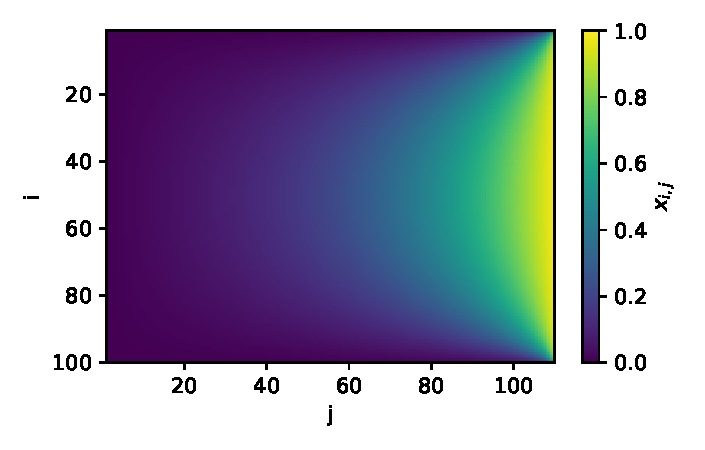
\includegraphics[width=0.55\linewidth]{figures/laplace.pdf}\]

\end{enumerate}
\end{minipage}

\end{enumerate}
%%%%%%%%%%%%%%%%%%%%%%%%%%%%%%%%%%%%%%%%%%%%%%%%%%%%%%
%                       End                          %
%%%%%%%%%%%%%%%%%%%%%%%%%%%%%%%%%%%%%%%%%%%%%%%%%%%%%%

\end{document}
